\documentclass[a4paper,12pt]{article}
\usepackage[utf8]{inputenc}

\usepackage[utf8]{inputenc}
\usepackage[T2A]{fontenc}
\usepackage[english,russian]{babel}
\usepackage{amsthm}
\usepackage{amsmath}
\usepackage{amssymb}
\usepackage{tikz}
\usepackage{textcomp}
\usepackage{marvosym}
\usepackage{ esint }
\usepackage{mathtext}
\usepackage{siunitx} % Required for alignment
\usepackage{subfigure}
\usepackage{multirow}
\usepackage{rotating}
\usepackage{afterpage}
\usepackage[arrowdel]{physics}
\usepackage{booktabs}
\setlength{\topmargin}{-0.5in}
\setlength{\textheight}{9.1in}
\setlength{\oddsidemargin}{-0.4in}
\setlength{\evensidemargin}{-0.4in}
\setlength{\textwidth}{7in}
\setlength{\parindent}{0ex}
\setlength{\parskip}{1ex}
\newcommand{\ndiv}{\hspace{-4pt}\not|\hspace{2pt}}
\usepackage{graphicx}
\usepackage{float}
\usepackage{wrapfig}
\usepackage{pgfplots}
\usepackage{caption}
\pgfplotsset{compat=1.16}
\graphicspath{ {./images/} }
\usepackage{graphicx}
\RequirePackage{caption}
\DeclareCaptionLabelSeparator{defffis}{ — }
\captionsetup{justification=centering,labelsep=defffis}
\usepackage{caption} \captionsetup[table]{labelsep=endash,justification=justified,singlelinecheck=false,font=normalsize}
\usepackage{amsfonts,mathtools}

\title{Лабораторная работа № 5.1.1\\Фотоэффект}
\author{Илья Прамский}
\date{Сентябрь 2024}

\begin{document}
\maketitle
\newpage
\section{Теоретическая справка}
Фотоэффект - испускание электронов фотокатодом, облучаемым светом - хорошо объясняется фотонной теорией света: фотон с энергией $\hbar \omega$ выбивает электрон из поверхности металла и сообщает электрону кинетическую энергию

Энергетический баланс этого взаимодействия описывается уравнением:
\begin{equation}
\hbar \omega = W + E_{max}
\end{equation}
где W - работа выхода электрона из катода, $E_{max}$ - максимальная кинетическая энергия электрона после выхода из фотокатода. Реально энергетический спектр вылетевших из фотокатода электронов непрерывный - он простирается от нуля до $E_{max}$.

Для измерения энергии вылетевших фотоэлектронов вблизи фотокатода располагают второй электрод(анод), на который подаётся потенциал. При достаточно большом ускоряющем напряжении(V>0) фототок достигает насыщения: все испущенные электроны попадают на анод. При некотором значении $V = -V_0$(потенциал запирания) даже наиболее быстрые фотоэлектроны не могут достичь анода. Данная зависимость изображена на рисунке 1.

\begin{figure}[H]
\centering
\includegraphics[scale=0.7]{ris1.png}
\end{figure}

Подставляя в 1 уравнение $E_{max} = eV_0$, получаем уравнение Эйнштейна для фотоэффекта:
\begin{equation}
eV_0 = \hbar \omega - W
\end{equation}

В самом простом случае, зависимость силы тока от напряжения $\sqrt{I} = f(V_0-V)$.

Для экспериментальной проверки уравнения Эйнштейна, по графикам данной зависимости определяются потенциалы запирания при разных частотах света и строится зависимость $V_0(/omega)$, которая должна иметь вид:
\begin{equation}
V_0(\omega) = \frac{\hbar \omega - W}{e}
\end{equation}
Получается, по наклону прямой можно найти постоянную Планка
\begin{equation}
\frac{dV_0}{d\omega} = \frac{\hbar}{e}
\end{equation}

\section{Экспериментальная  установка}
Схема установки приведена на рисунке 2. Свет от источника S с помощью конденсора фокусируется на входную щель призменного монохроматора УМ-2, выделяющего узкий спектральный интервал, и попадает на катод фотоэлемента Ф-25

%\begin{figure}[H]
%\begin{minipage}
%\includegraphics[scale=0.8]{scheme1.png}
%\end{minipage}
%\begin{minipage}
%\includegraphics[scale=0.8]{scheme2.png}
%\end{minipage}
%\caption*{Рис. 2. Схема экспериментальной установки Рис. 3. Схема монохроматора}
%\end{figure}

\begin{figure}[H]
  \centering
  \begin{minipage}[b]{0.45\textwidth}
    \includegraphics[width=\textwidth]{scheme1.png}
    \caption*{Рис. 2. Схема экспериментальной установки}
  \end{minipage}
  \hfill
  \begin{minipage}[b]{0.45\textwidth}
    \includegraphics[width=\textwidth]{scheme2.png}
    \caption*{Рис. 3. Схема монохроматора}
  \end{minipage}
\end{figure}

Основные элементы монохроматора представлены на рисунке 3.

Входная щель 1 с микрометрическим винтом 9 для её открытия на нужную ширину(0,01 - 4 мм).

Коллиматорный объектив 2 с микрометрическим винтом 8, что позволяет смещать объектив относительно щели

Система призм 3, предназначенная для выделения частоты и поворота лучей на 90 градусов

Поворотный столик 6 с винтом 7 для вращения барабана с целью поворота призмы, чтобы в поле зрения были другие участки спектра

Зрительная труба с объективом 4, окуляром 5, острием указателя 10. 

Корпус 10, оптическая скамья длярасположения линзы и источника, пульт управления.

\section{Ход работы}
Для начала подготовим установку к работе. Для этого расположим неоновую лампу и линзу на оптическую скамью, настроим их так, чтобы свет попадал на входную щель. Далее откроем входную щель, включим подсветку окуляра и настроимся на чёткое изображение кончика указателя. Далее, для улучшения точности, вращая винт 8, настроим изображение спектра света так, чтобы избежать параллакса света и кончика указателя. Установка подготовлена к работе.

\subsection*{Градуировка монохроматора}
Пользуясь таблицой из методических материалом, проградуируем барабан монохроматора по спектру неоновой лампы. Для этого построим( по известным из таблицы данным и полученной информации об углах из эксперимента) график зависимости длины волны света от угла на барабане.


\begin{table}[H]
    \centering
    \begin{tabular}{|c|c|c|c|c|c|c|c|c|c|c|c|c|c|}
    \hline
      $\lambda,$ \AA   & 5331 & 5341 & 5401 & 5852 & 5882 & 5945 & 5976 & 6030 & 6074 & 6096 & 6143 & 6164 & 6217\\
      \hline
      $\varphi$   & 2205 & 2212 & 2254 & 2513 & 2529 & 2560 & 2574 & 2600 & 2618 & 2628 & 2649 & 2658 & 2682\\
    \hline      
    $\lambda,$ \AA   & 6267 & 6305 & 6334 & 6383 & 6402 & 6507 & 6533 & 6599 & 6678 & 6717 & 6929 & 7032 &\\
      \hline
      $\varphi$ & 2702 & 2719 & 2731 & 2750 & 2759 & 2798 & 2806 & 2833 & 2860 & 2873 & 2944 & 2972 & \\
    \hline
    		
    \end{tabular}
    \caption{Таблица с длинами волн полос спектра и соответствующими им углами на барабане}
    \label{Таблица с длинами волн полос спектра и соответствующими им углами на барабане}
\end{table}
\begin{figure}[H]
\centering
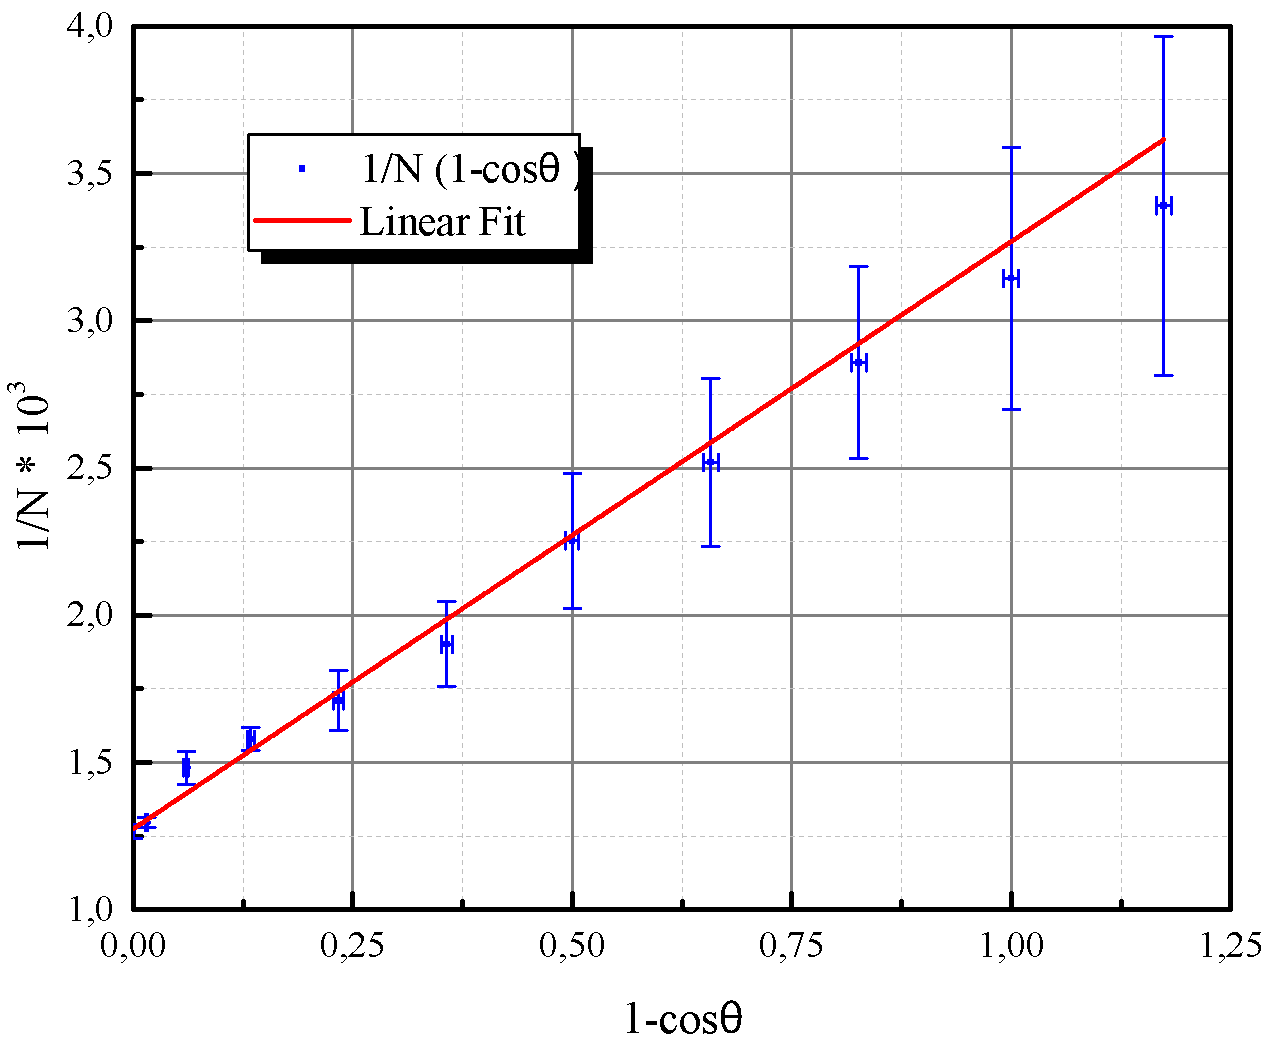
\includegraphics[scale=1]{graph1.png}
\end{figure}

\subsection*{Исследование зависимости фототока от величины запирающего потенциала}

Установим вместо неоновой лампы электрическую, настроим её на резкое изображение на входной щели, затем установим показания вольтметра близким к нулю при закрытом входе монохроматора. После этого откроем входную щель.

Теперь же измерим зависимость фототока от напряжения. В моём случае установка была неисправна, из-за чего при выставлении какого-то фиксированного значения напряжения V, фототок со временем стремительно увеличивался. В связи с этим реальная зависимость стала больше похожей на линейную

По указанию преподавателя, я рассмотрел зависимость, как линейную(I = f(V)), но получил различие со справочными данными на несколько порядков, из-за чего я решил взять данные по данному пункту у одногруппник. Рассмотрев как изменяется фототок в зависимости от напряжения, построим графики зависимости $\sqrt{I} = f(V)$ для 5 разных частот и для каждой из них найдём значение запирающего потенциала.

\vspace{5mm}
\begin{table}[H]

\begin{tabular}{|c|c|c|c|c|c|c|c|c|c|c|c|}
\hline
\multicolumn{12}{|c|}{$\lambda$, \AA} \\
\hline
\multicolumn{2}{|c|}{5331} & \multicolumn{2}{|c|}{5852} & \multicolumn{2}{|c|}{6074} & \multicolumn{2}{|c|}{6334} & \multicolumn{2}{|c|}{6599} & \multicolumn{2}{|c|}{7032} \\
\hline
$\sqrt{I}, A^\frac{1}{2}$,  & $V$, В & $\sqrt{I}$, $A^\frac{1}{2}$ & $V$, В & $\sqrt{I}$, $A^\frac{1}{2}$ & $V$, В & $\sqrt{I}$, $A^\frac{1}{2}$ & $V$, В & $\sqrt{I}$, $A^\frac{1}{2}$ & $V$, В & $\sqrt{I}$, $A^\frac{1}{2}$ & $V$, В \\
\hline
0,32 & 0,70 & 0,32 & 0,35 & 0,32 & 0,30 & 0,32 & 0,34 & 0,32 & 0,32 & 0,32 & 0,38 \\
\hline
0,39 & 1,17 & 0,39 & 0,62 & 0,39 & 0,52 & 0,39 & 0,52 & 0,39 & 0,48 & 0,39 & 0,51 \\
\hline
0,45 & 1,58 & 0,45 & 0,87 & 0,45 & 0,80 & 0,45 & 0,68 & 0,45 & 0,62 & 0,45 & 0,65 \\
\hline
0,50 & 2,00 & 0,50 & 1,11 & 0,50 & 1,05 & 0,50 & 0,86 & 0,50 & 0,77 & 0,50 & 0,78 \\
\hline
0,55 & 2,46 & 0,55 & 1,39 & 0,55 & 1,22 & 0,55 & 1,05 & 0,55 & 0,94 & 0,55 & 0,93 \\
\hline

\end{tabular}
\end{table}

\begin{figure}[H]
\centering
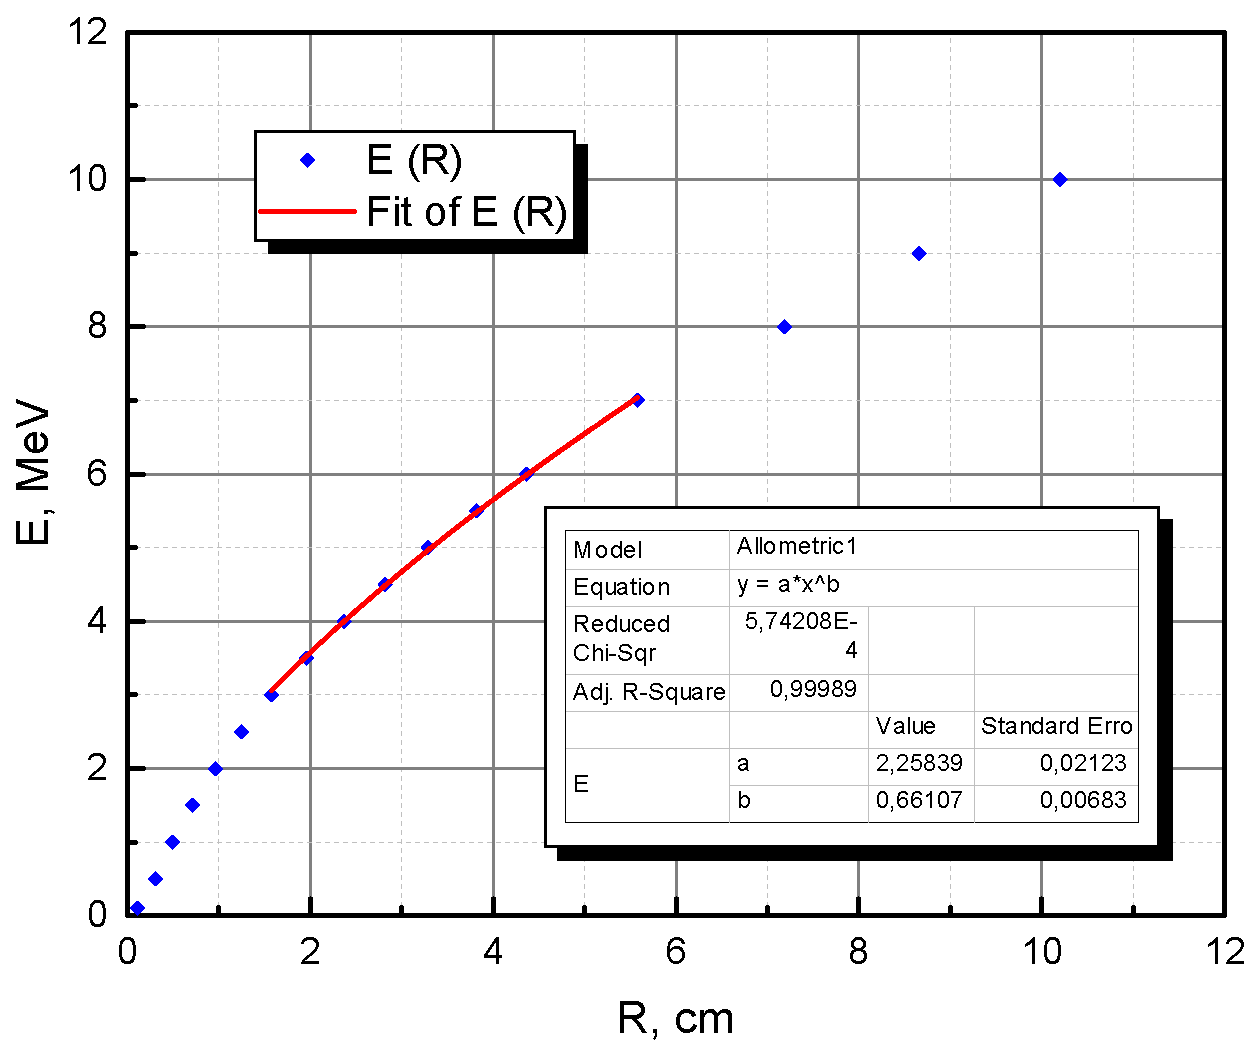
\includegraphics[scale=0.73]{graph4.png}
\end{figure}

\begin{figure}[H]
  \centering
  \begin{minipage}[b]{0.48\textwidth}
    \includegraphics[width=\textwidth]{line1.png}
  \end{minipage}
  \hfill
  \begin{minipage}[b]{0.48\textwidth}
    \includegraphics[width=\textwidth]{line2.png}
  \end{minipage}
  \hfill
  \begin{minipage}[b]{0.48\textwidth}
    \includegraphics[width=\textwidth]{line3.png}
  \end{minipage}
  \hfill
  \begin{minipage}[b]{0.48\textwidth}
    \includegraphics[width=\textwidth]{line4.png}
  \end{minipage}
  \hfill
  \begin{minipage}[b]{0.48\textwidth}
    \includegraphics[width=\textwidth]{line5.png}
  \end{minipage}
  \hfill
  \begin{minipage}[b]{0.48\textwidth}
    \includegraphics[width=\textwidth]{line6.png}
  \end{minipage}
\end{figure}

\begin{figure}[H]
\centering
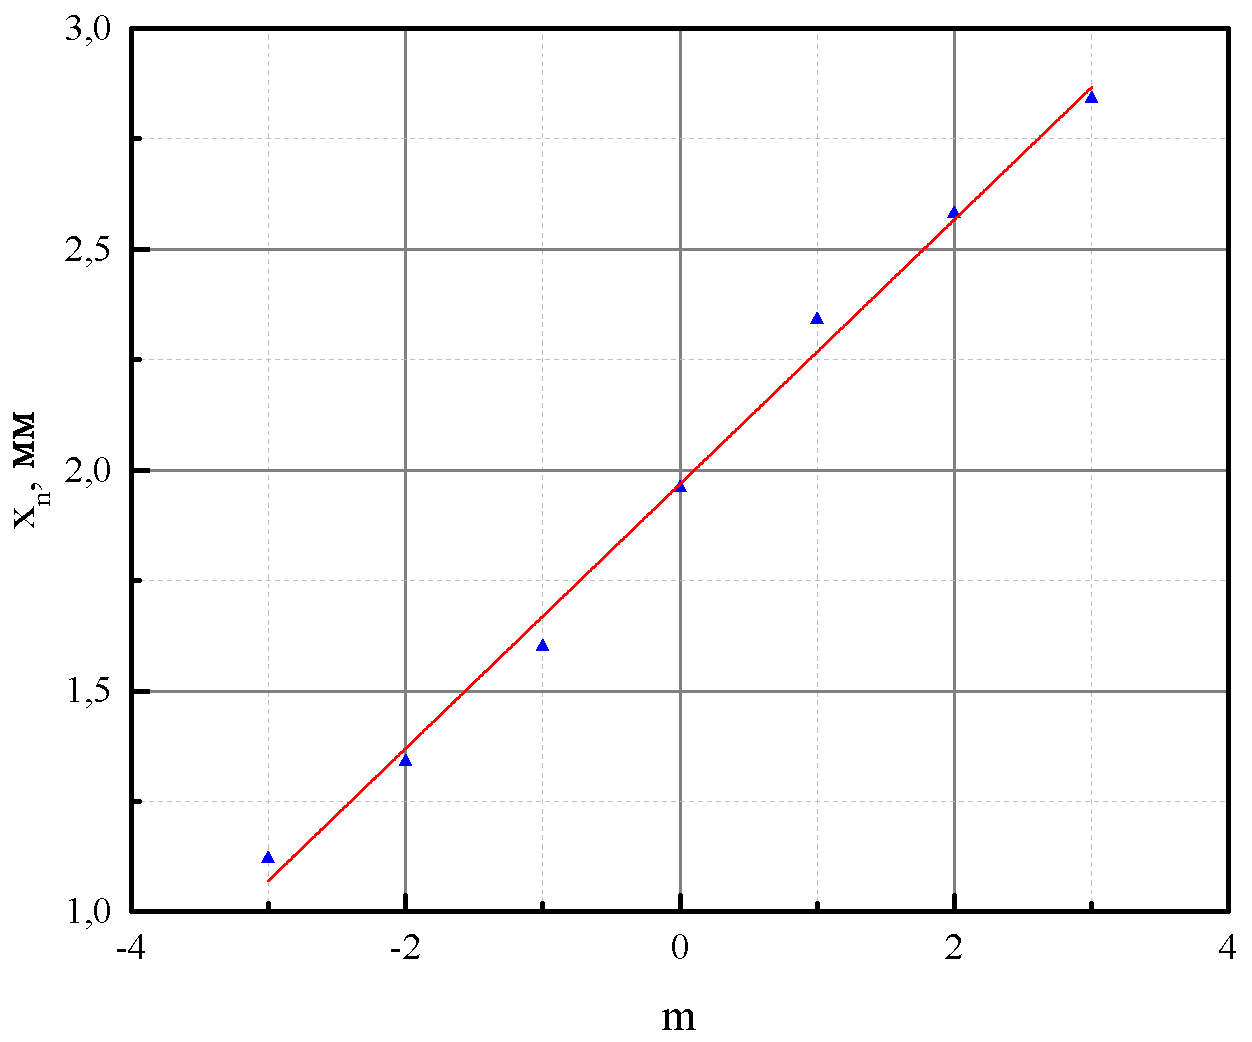
\includegraphics[scale=0.8]{graph2.png}
\end{figure}

Найдём коэффициенты k и b для полученных линейных зависимостей, а затем, приравняв фототок к нулю, найдём потенциал насыщения.

\begin{table}[H]
\centering
\begin{tabular}{|c|c|c|c|c|c|c|}
\hline
$\lambda$, \AA & $k, \frac{A^\frac{1}{2}}{B}$ & $\sigma_k, \frac{A^\frac{1}{2}}{B}$ & $b, A^\frac{1}{2}$ & $\sigma_b, A^\frac{1}{2}$ & $V_0, B$ & $\sigma_{V_0}, B$ \\
\hline
5331 & 0,132 & 0,006 & 0,23 & 0,01 & 1,74 & 0,11 \\
\hline
5852 & 0,222 & 0,011 & 0,25 & 0,01 & 1,11 & 0,07 \\
\hline
6074 & 0,242 & 0,011 & 0,25 & 0,01 & 1,04 & 0,06\\
\hline
6334 & 0,328 & 0,019 & 0,21 & 0,01 & 0,65 & 0,06\\
\hline
6559 & 0,370 & 0,020 & 0,21 & 0,01 & 0,55 & 0,05 \\
\hline
7032 & 0,420 & 0,020 & 0,17 & 0,02 & 0,39 & 0,05\\
\hline 

\end{tabular}
\end{table}
\newpage
Далее построим график зависимости $V_0 = f(\omega)$. Получилось

\begin{figure}[H]
\centering
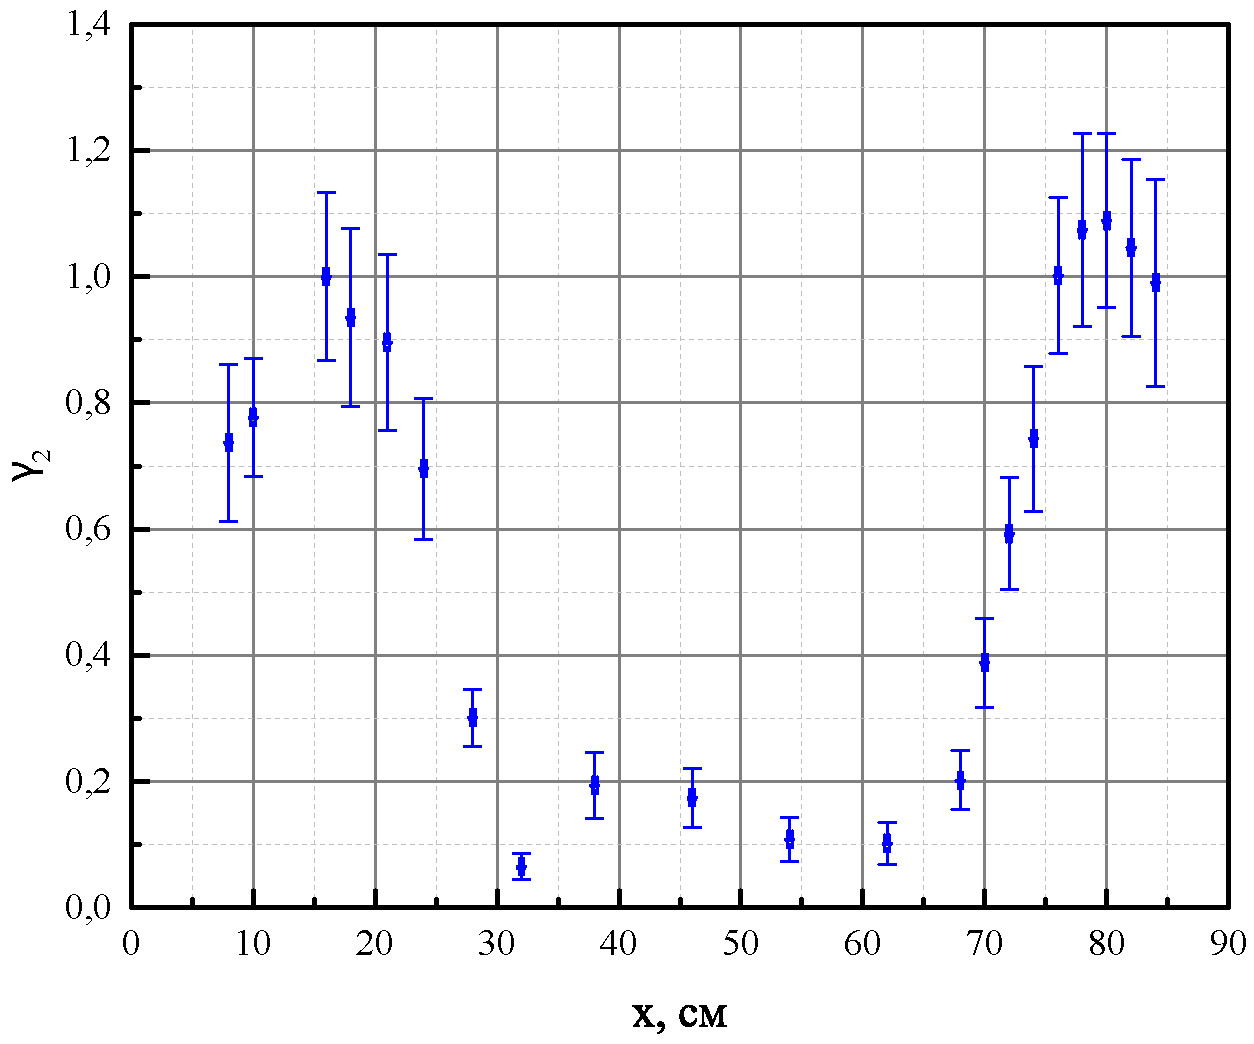
\includegraphics[scale=0.8]{graph3.png}
\end{figure}

Получается, $k = \frac{\hbar}{e} = 1,62 \pm 0,15 \cdot 10^{-15} \frac{\text{Дж} \cdot c}{\text{Кл}}$. $\hbar = 2,6 \pm 0,2 \cdot 10^{-34} \text{Дж} \cdot c$.

\section{Вывод}
В ходе данной работы было исследовано явление фотоэффекта, проверена справедливость уравнения Эйнштейна для фотоэффекта при помощи рассмотрения зависимостей, которые она задаёт между величинами. Получившееся значение $\frac{\hbar}{e} = 1,62 \pm 0,15 \cdot 10^{-15} \frac{\text{Дж} \cdot c}{\text{Кл}}$, теоретическое же равно $6,57 \cdot 10^{-16} \frac{\text{Дж} \cdot c}{\text{Кл}}$.


\end{document}